\documentclass[a4paper,11pt,french]{article}
\usepackage[utf8]{inputenc}

\usepackage[T1]{fontenc}
\usepackage[francais]{babel} 
\usepackage[top=2cm, bottom=2cm, left=2cm, right=2cm, includeheadfoot]{geometry} %pour les marges
\usepackage{lmodern}
\usepackage{pict2e}
\usepackage{fancyhdr} % Required for custom headers
\usepackage{lastpage} % Required to determine the last page for the footer
\usepackage{extramarks} % Required for headers and footers
\usepackage{graphicx} % Required to insert images
\usepackage{tabularx, longtable}
\usepackage{color, colortbl}
\usepackage{lscape}
%\usepackage[hidelinks]{hyperref}
\usepackage{longtable}
\usepackage{multirow}
\usepackage{rotating}
\usepackage{gensymb}
\usepackage{soulutf8}

\linespread{1.1} % Line spacing

% Set up the header and footer
\pagestyle{fancy}
\lhead{\textbf{\hmwkClass -- \hmwkSubject \\ \hmwkTitle \\ \hmwkDocName}} % Top left header
\rhead{
\includegraphics[width=10em]{../images/logo_univ.png}}
\lfoot{\lastxmark} % Bottom left footer
\cfoot{} % Bottom center footer
\rfoot{Page\ \thepage\ / \pageref{LastPage}} % Bottom right footer
\renewcommand\headrulewidth{0.4pt} % Size of the header rule
\renewcommand\footrulewidth{0.4pt} % Size of the footer rule

\setlength{\headheight}{40pt}

\newcommand{\hmwkTitle}{Transchiffrement} % Assignment title
\newcommand{\hmwkClass}{Master 2 SSI } % Course/class
\newcommand{\hmwkAuthorName}{Julien BOURDON, Émile GÉNÉRAT} % Your name
\newcommand{\hmwkSubject}{Conduite de projet} % Subject
\newcommand{\hmwkDocName}{Spécification Technique du Besoin} % Document name

\newcommand{\version}{1.4} % Document version
\newcommand{\docDate}{24 février 2014} % Document date
\newcommand{\checked}{Jean-Baptiste SOUCHAL} % Checker name
\newcommand{\approved}{} % Approver name

\makeatletter
\newcommand{\resettranslate}{\let\translate\@firstofone}
\makeatother

\definecolor{gris}{rgb}{0.95, 0.95, 0.95}

\title{
\vspace{2in}
\textmd{\textbf{\hmwkClass :\ \hmwkTitle}}\\
\normalsize\vspace{0.1in}\small{Due\ on\ \hmwkDueDate}\\
\vspace{0.1in}\large{\textit{\hmwkClassInstructor\ \hmwkClassTime}}
\vspace{3in}
}

\author{\hmwkAuthorName}
\date{} % Insert date here if you want it to appear below your name


\usepackage{amsmath}
\begin{document}
\newcount\startdate
\newcount\daynum
%\pgfcalendardatetojulian{2013-01-021}{\startdate}
\pagestyle{fancy}

\vspace*{5cm}
\begin{center}\textbf{\Huge{\hmwkDocName}}\end{center}
\vspace*{4.5cm}
	

\fcolorbox{black}{gris}{
\begin{minipage}{15cm}
\begin{tabularx}{10cm}{lXl}
	\bfseries{Version} & & \version\\
	& & \\
	\bfseries{Date} & & \docDate\\
	& & \\
	\bfseries{Rédigé par} & & \hmwkAuthorName \\
	& & \\
	\bfseries{Relu par} & & \checked \\
	& & \\
	\bfseries{Approuvé par} & & \approved \\
	& & \\
\end{tabularx}
\end{minipage}
}

\newpage

%Tableau de mises à jour
\vspace*{1cm}
\begin{center}
\textbf{\huge{Versions}}\\
\vspace*{3cm}
	\begin{tabularx}{16cm}{|c|c|X|}
	\hline
	\bfseries{Version} & \bfseries{Date} & \bfseries{Modifications réalisées}\\
	\hline
	1.0 & 27/11/2013 & Création\\
	\hline
	1.1 & 22/01/2014 & Prise en compte des remarques suite aux réunions client et à l'audit.\\
	\hline
	1.2 & 27/01/2014 & Prise en compte des nouvelles remarques du client.\\
	\hline
	1.3 & 06/02/2014 & Correction de fautes.\\
	\hline
	1.4 & 24/02/2014 & Modification d'un cas d'exception.\\
	\hline
	\end{tabularx}
\end{center}

%La table des matières
\clearpage
\tableofcontents
\clearpage


\newpage
\section{Présentation de la mission du produit logiciel}

Dans le cadre de notre projet professionnel de dernière année de Master en Sécurité des Systèmes 
Informatiques, nous avons réalisé le projet "Transchiffrement SSL" qui s'articule sur deux axes. Un proxy de transchiffrement SSL, suivi d'une 
étude sur la collision de certificats de type MD5.

Ce projet a fait l'objet d'une étude en amont pour préparer la phase de 
développement. Cette étude nous a permis d'avoir une vision d'ensemble du projet 
ainsi qu'un listing détaillé de toutes les tâches à réalisées lors de la phase 
de développement.~~\\

Pour garantir la confidentialité du trafic internet, les sites ont de plus en plus souvent recours au chiffrement des échanges en utilisant le protocole HTTPS.
Ce chiffrement s'effectue de bout en bout, du client jusqu'au serveur à l'aide d'un tunnel SSL.
Ainsi, un intrus qui intercepte les connexions ne peut pas lire les paquets qui transitent.


Fréquemment, les entreprises analysent le trafic entrant et sortant de leur réseau.
Cette analyse du contenu des paquets, grâce à des IDS par exemple, permet de rechercher la présence de virus,
malware ou autres comportements suspect sur un réseau non sécurisé. Or de plus en plus, les 
logiciels malveillants utilisent le protocole HTTPS pour s'introduire dans un 
réseau. L'utilisation de ce protocole rend inutile toutes les techniques 
d'écoute sur un réseau non sécurisé.


Le but du projet est de fournir une solution de transchiffrement SSL, qui permette d'analyse en clair au sein du proxy les paquets,
qu'ils soient issus d'une connexion en clair ou chiffrée. Dans ce dernier cas, il faut établir une connexion chiffrée vers le client,
et une autre vers le serveur distant à partir du proxy de transchiffrement.
La mise en place d'un tel dispositif est à double tranchant, d'un côté il permet 
l'analyse du trafic HTTPS pour la détection de logiciels malveillants et donc la 
sécurisation d'un réseau, mais de façon contradictoire il permet "l'espionnage" 
des données échangées lors d'une connexion normalement secrète.

Ce système permet donc de faire une attaque de type "Man In The Middle" du point 
du vue défensif, pour l'analyse du réseau ou du point de vue attaquant pour 
l'espionnage des données.
~~\\

La deuxième partie du projet porte sur l'étude de collisions sur des certificats
de type MD5. Le but d'une telle collision est donc de forger un faux certificat 
ayant exactement la même signature que l'original. Ainsi un navigateur web ne 
fera aucune différence avec le certificat original et le faux certificat, les 
deux seront reconnus comme valide auprès de l'autorité de certification du serveur 
web.



Les trois méthodes attendues par le client sont :
\begin{itemize}
\item Installer directement notre autorité de certification dans le système.
\item Forcer l'utilisateur à accepter notre autorité de certification.
\item Forger un faux certificat d'autorité qui a le même haché MD5 qu'un certificat d'autorité valide existant.
\end{itemize}

\hl{La dernière méthode nécessite des recherches spécifiques, pour comprendre et mettre en oeuvre des collisions entre deux certificats.}


Une fois l'autorité installée et acceptée, nous l'utiliserons pour signer les certificats des serveurs auxquels le client veut se connecter que nous créerons à la volée. Une fois créés, nous pourrons les stocker pour une éventuelle réutilisation, ce qui nous fera gagner du temps.


\hl{La vitesse d'exécution est un exigence non-fonctionnelle importante pour éviter que les utilisateurs aient des doutes.}

La deuxième partie du projet est surtout un travail de recherche sur les collisions MD5 afin de trouver un algorithme qui nous permette de forger cette fausse autorité. Nous aurons donc à faire tourner un programme de comparaison pendant une durée assez longue en parallèle de la première partie du projet.

\subsection{Terminologie}

\begin{description}
\item[Client] Utilisateur d'une machine privée (ordinateur) qui souhaite se connecter à un serveur \hl{sur Internet}.
\item[Proxy] \hl{Machine intermédiaire qui écoute sur le réseau, qui va transférer les trames après analyse, et si nécessaire réaliser le transchiffrement TLS/SSL.}
\item[Serveur] Machine sur Internet accessible à partir d'une URL ou d'une adresse IP.
\item[Certificat] \hl{Fichier qui prouve l'appartenance d'une clé publique à un individu.}
\item[Autorité de certification] \hl{Autorité qui utilise sa clé privée pour signer des certificats.}

\end{description}

\subsection{Liste des cas d'utilisation}

Les différents cas d'utilisation de l'application sont les suivants.

\begin{center}
\begin{tabular}{|l|m{12cm}|l|}
\hline 
\rowcolor[gray]{.8} ID & Intitulé & Priorité \\ 
\hline
P.1 & Navigation en clair & Indispensable\\
\hline
P.2 & Installation de SSI-Cert par un administrateur sur la machine client  & Indispensable \\ 
 \hline 
P.3 & Installation de SSI-Cert par l'utilisateur dans son navigateur
 & Indispensable \\ 
\hline 
P.4 & Signature de Fake-Cert avec SSI-Cert-Collision dont le haché MD5 est le même que International-Cert accepté par la machine client & Optionnel \\
\hline
P.5 & Génération d'un certificat serveur Fake-Cert & Indispensable \\ 
\hline
P.6 & Établissement d'une connexion SSL/TLS & Indispensable \\
\hline
P.7 & Navigation SSL/TLS & Indispensable \\ 
\hline

 

\end{tabular} 
\end{center}
~~\\
\textbf{Exigence fonctionnelle indispensable :} Étude recherche de collsion MD5
~~\\

\huge
\subsection{Diagramme UML}
\begin{center}
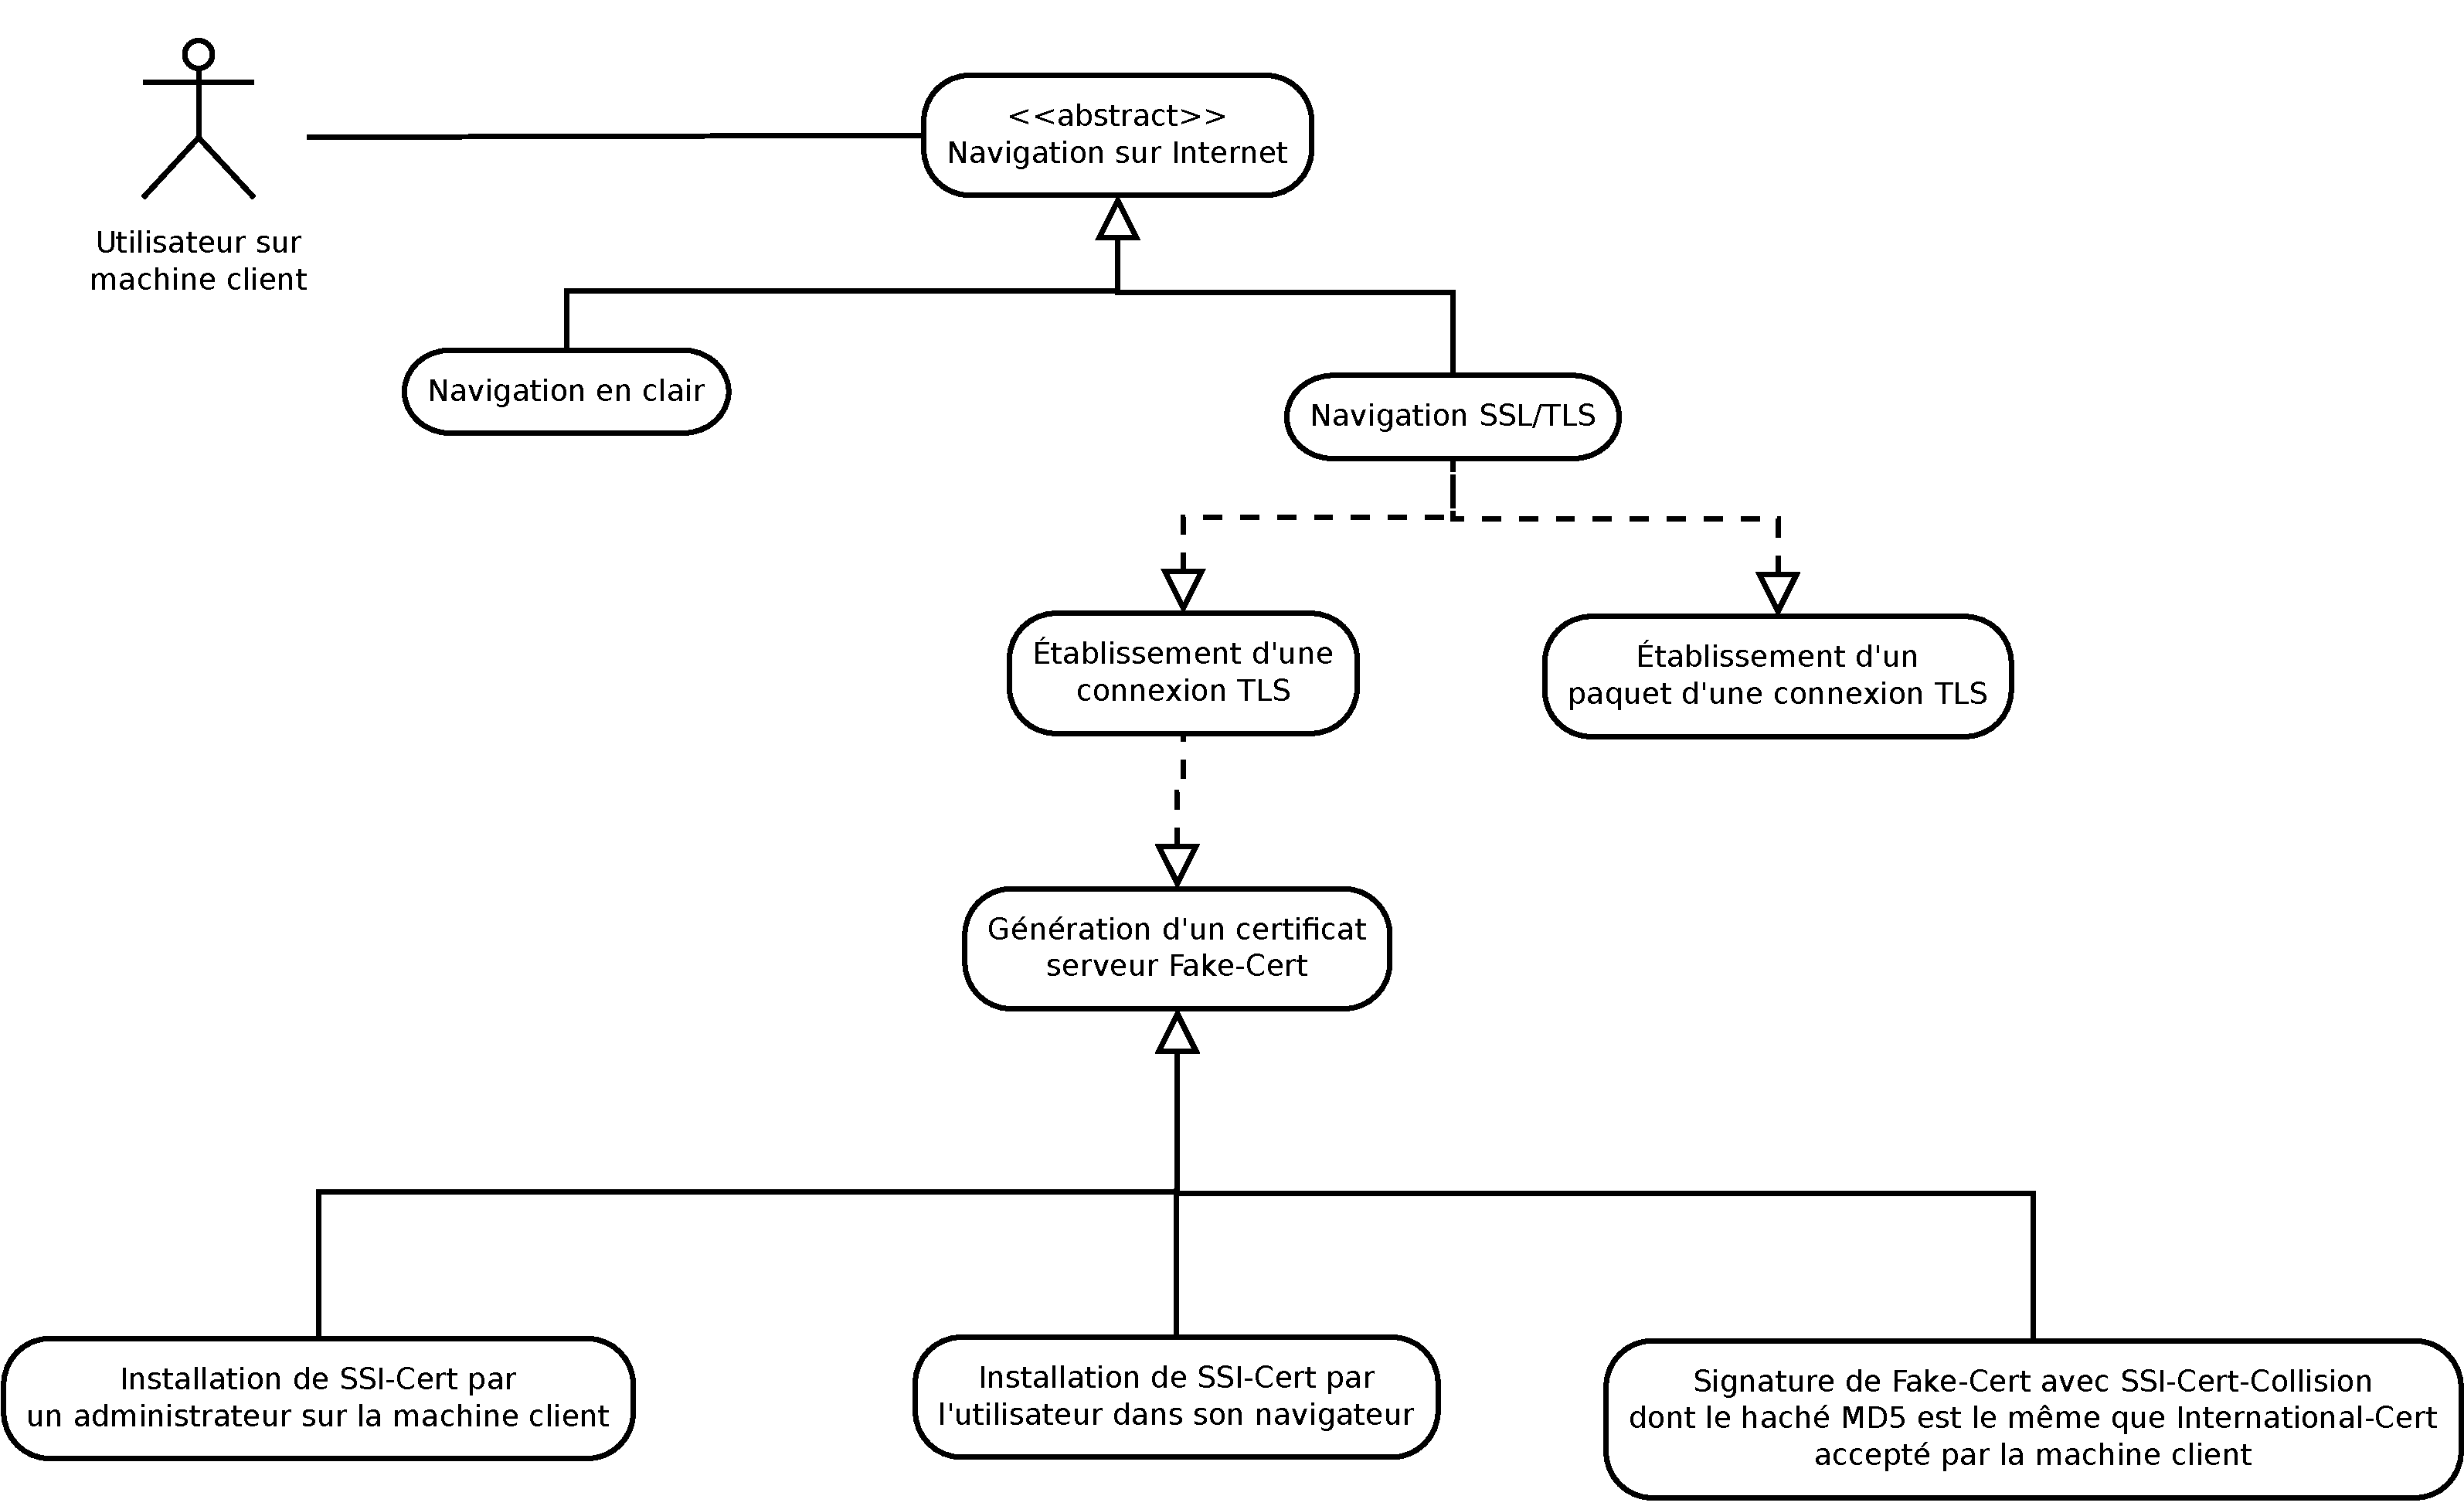
\includegraphics[width=\textwidth]{images/cas_utilisation.pdf}
\end{center}
\normalsize


\section{Cas d'utilisation}

\subsection{Navigation en clair}
\begin{tabular}{|>{\columncolor[gray]{.8}}m{4cm}|m{12cm}|}
   \hline
   Description & Transfert de trames en clair  \\
   \hline
   Pré-conditions & Connexion non-sécurisée établie \\
   \hline
   Évènement déclenchant &  Réception d'une trame en clair sur une interface. \\
   \hline
   Condition d'arrêt & Trame transférée sur l'autre interface. \\
   \hline
   Cas d'exception  &  \\
   \hline   
\end{tabular}
~\\
Description du flot d'évènements principal :

\begin{tabular}{|m{8cm}|m{8cm}|}
   \hline
  \rowcolor[gray]{.8} Acteur(s) & Système \\
   \hline
   1. Envoi d'une trame en clair par le client ou le serveur. & \\
   \hline
&   2. Réception par le proxy.  \\
   \hline   
 &     3. Le proxy journalise le paquet.  \\
      \hline
&      4. Le proxy retransmet le paquet au destinataire.  \\
   \hline
\end{tabular}

\subsection{Installation de SSI-Cert par un administrateur sur la machine client}
Dans ce cas de figure, on prend l'exemple d'un administrateur système qui installe directement l'autorité sur les machines clientes.

\begin{tabular}{|>{\columncolor[gray]{.8}}m{4cm}|m{12cm}|}

   \hline
   Description & Première façon de faire : installer directement l'autorité dans le système\\
   \hline
   Pré-conditions &Autorité par défaut présente \\
   \hline
   Évènement déclenchant &  Mise en place de l'autorité\\
   \hline
   Condition d'arrêt & Autorité SSI-Sign reconnue comme valide \\
   \hline
   Cas d'exception  & \\
   \hline   
\end{tabular}


~\\

Description du flot d'évènements principal :

\begin{tabular}{|m{8cm}|m{8cm}|}
   \hline
   \rowcolor[gray]{.8} Acteur(s) & Système \\
   \hline
   1. Installation de l'autorité directement dans le système du client. & \\
   \hline
\end{tabular}



\newpage
\subsection{Installation de SSI-Cert par l'utilisateur dans son navigateur}
\begin{tabular}{|>{\columncolor[gray]{.8}}m{4cm}|m{12cm}|}
   \hline
   Description & Lors de sa connexion au proxy, on force l'utilisateur à accepter le SSI-Cert. \\
   \hline
   Pré-conditions &  \\
   \hline
   Évènement déclenchant & Première connexion au proxy par le client \\
   \hline
   Condition d'arrêt & Autorité SSI-Sign reconnue comme valide. \\
   \hline
   Cas d'exception  &  \\
   \hline   
\end{tabular}

~\\

Description du flot d'évènements principal :

\begin{tabular}{|m{8cm}|m{8cm}|}
   \hline
  \rowcolor[gray]{.8} Acteur(s) & Système \\
   \hline
   1. Le client se connecte au proxy. & \\
   \hline
    & 2. Le client est redirigé vers une page de téléchargement de SSI-Cert. \\
   \hline
   3. Le client accepte SSI-Cert. &  \\
   \hline
\end{tabular}



\subsection{Signature de Fake-Cert avec SSI-Cert-Collision dont le haché MD5 est le même que International-Cert accepté par la machine client }
\begin{tabular}{|>{\columncolor[gray]{.8}}m{4cm}|m{12cm}|}
   \hline
   Description & Utilisation d'un certificat généré à partir d'une collision. \\
   \hline
   Pré-conditions & \begin{itemize}
\item  L'étude a permis d'obtenir un deuxième certificat de même haché MD5, mais dont on connaît la clé privée associée.
  \item Le client possède l'autorité attaquée.
   \end{itemize} \\
   \hline
   Évènement déclenchant & Un client demande une connexion. \\
   \hline
   Condition d'arrêt & Le certificat Fake-Cert est reconnu valide par le client. \\
   \hline
   Cas d'exception  &  \\
   \hline   
\end{tabular}

~\\

Description du flot d'évènements principal :

\begin{tabular}{|m{8cm}|m{8cm}|}
   \hline
  \rowcolor[gray]{.8} Acteur(s) & Système \\
   \hline
   1. Le client demande une connexion à un serveur. & \\
   \hline
&    2. Le proxy demande une connexion à ce serveur et récupère son certificat Site-Cert.  \\
   \hline
   &    3. Le proxy génère Fake-Cert à partir de Site-Cert et le signe avec SSI-Sign-Collision.  \\
   \hline
   &    4. Le proxy établit une connexion SSL/TLS avec le client en utilisant Fake-Cert.  \\
   \hline
 Le client reconnaît Fake-Cert comme valide, car la signature de SSI-Cert-Collision est valide (dupliquée d'un certificat de même haché) & \\
\hline
\end{tabular}

\subsection{Génération d'un certificat serveur Fake-Cert}
À chaque demande de connexion SSL/TLS du client à un serveur, un faux certificat est envoyé au client. Il est généré si nécessaire.

Ce cas d'utilisation peut être décliné avec deux autorités, SSI-Sign, et SSI-Sign-Collision si nous avons trouvé une collision entre deux certificats.

Le proxy ne peut utiliser qu'une des deux autorités, sélectionnée manuellement lors de l'installation du proxy.

\begin{tabular}{|>{\columncolor[gray]{.8}}m{4cm}|m{12cm}|}
   \hline
   Description & Génération de Fake-Cert à destination du client. \\
   \hline
   Pré-conditions & \begin{itemize}
\item Le proxy est configuré sur le client.
\item Le proxy est lancé.
\item SSI-Cert est accepté par le client.
   \end{itemize}
 \\
   \hline
   Évènement déclenchant & Le client tente de se connecter à un serveur \\
   \hline
   Condition d'arrêt &  Fake-Cert et la chaîne de certification avec SSI-Cert sont envoyés au client. \\
   \hline
   Cas d'exception  &
\\
   \hline   
\end{tabular}

~\\

Description du flot d'évènements principal :

\begin{tabular}{|m{8cm}|m{8cm}|}
   \hline
  \rowcolor[gray]{.8} Acteur(s) & Système \\
   \hline
   1. Le client tente de se connecter à un serveur & \\
   \hline
    & 
2. 
Deux cas sont possibles :
\begin{itemize}
\item Si le certificat est déjà dans la base de données, on le récupère.
\item Sinon Fake-Cert est généré :
\begin{itemize}
\item Le issuer est SSI-Sign.
\item La clé publique est celle du bi-clé Fake-Cert, elle est constante pour tous les Fake-Cert. Nous connaissons la clé privée.
\end{itemize}
\end{itemize}
3. On envoie Fake-Cert au client. \\
   \hline
   4. Le client reconnaît Fake-Cert comme valide, car il est signé par SSI-Sign. &  \\
   \hline
\end{tabular}

\subsection{Établissement d'une connexion SSL/TLS}
\begin{tabular}{|>{\columncolor[gray]{.8}}m{4cm}|m{12cm}|}
   \hline
   Description & Transfert des paquets chiffrés \\
   \hline
   Pré-conditions & Connexion SSL/TLS établie \\
   \hline
   Évènement déclenchant &  Envoi d'un paquet chiffré du client vers le serveur. \\
   \hline
   Condition d'arrêt & Réponse chiffrée du serveur transmise au client. \\
   \hline
   Cas d'exception  & Le client n'a pas accepté SSI-Cert. \\
   \hline   
\end{tabular}
~\\
Description du flot d'évènements principal :

Dans ce cas d'utilisation, nous modifions les acteurs : le client est à gauche, le serveur à droite.

Pour établir une connexion, il faut établir deux connexions SSL/TLS, une de chaque côté.

Le proxy jouera alternativement les rôles de client et serveur.

\begin{tabular}{|m{8cm}|m{8cm}|}
   \hline
  \rowcolor[gray]{.8} Client & Serveur \\
   \hline
1. (Client Hello) : Contient la date, un nonce et les algorithmes disponibles. & \\
   \hline
&2. (Server Hello) : Contient la date, un nonce et l'algorithme choisi.\\
   \hline
& 3. (Server Certificate) :  Contient un Site-Cert ainsi que les certificats de la chaîne de certification (Autorité).\\
   \hline
& 4. (Client Certificate Request) : Optionnel, seulement si le serveur veut que le client soit authentifié.\\
   \hline
& 5. (Server Hello Done) : Indique la fin d'envoi du serveur.\\
   \hline
6. (Client Certificate) : Si (4) est demandé, alors le client envoie son certificat. & \\
   \hline
7. (Client Key Exchange) : Paquet chiffré avec la clé publique du serveur qui contient une clé de session générée à partir des deux nonces échangés (Diffie-Hellman). Si le serveur est capable de déchiffrer et de répondre, il est authentifié auprès du client. & \\
   \hline
8. (Client Verify) : Si (4) est demandé, le client devra signer avec sa clé privée un haché des échanges précédents, ce qui l'authentifiera auprès du serveur. & \\
   \hline
9. (Change Cipher Spec.) : Précise que tous les paquets envoyés à la suite du "Client Finished" seront chiffrés avec la clé de session échangée et les algorithmes choisis. & \\
   \hline
10. (Client Finished) : Informe que le client a fini et contient un haché de la totalité des échanges. & \\
   \hline
& 11. (Change Cipher Spec.) : Précise qu'à partir de maintenant, le serveur va envoyer des paquets chiffrés. \\
   \hline
& 12. (Server Finished) : Contient un haché de tous les échanges chiffré avec la clé de session et un MAC.\\
   \hline
\end{tabular}


\newpage
\subsection{Navigation SSL/TLS}

\begin{tabular}{|>{\columncolor[gray]{.8}}m{4cm}|m{12cm}|}
   \hline
   Description & Transfert des paquets chiffrés \\
   \hline
   Pré-conditions & Connexion SSL/TLS établie \\
   \hline
   Évènement déclenchant &  Envoi d'un paquet chiffré du client vers le serveur. \\
   \hline
   Condition d'arrêt & Réponse chiffrée du serveur transmise au client. \\
   \hline
   Cas d'exception  & Le client n'a pas accepté SSI-Cert. \\
   \hline   
\end{tabular}
~\\
Description du flot d'évènements principal :

\begin{tabular}{|m{8cm}|m{8cm}|}
   \hline
  \rowcolor[gray]{.8} Acteur(s) & Système \\
   \hline
   1. Envoi d'un paquet Application-data chiffré du client vers le serveur& \\
   \hline
& 2. Le proxy déchiffre le paquet reçu à l'aide de la clé privée associée à Fake-Cert. \\
& 3. Le proxy chiffre le paquet avec la clé publique de Site-Cert.  \\
   \hline
 & 4. Transmission du paquet au serveur. \\
   \hline
5. Le serveur envoie sa réponse chiffrée avec la clé publique de Fake-Cert. &  \\
   \hline
  &  6. Le proxy déchiffre avec la clé privée de Fake-Cert, et rechiffre avec la clé publique du client.   \\
   \hline
      7. Le client déchiffre avec sa clé privée. &  \\
   \hline
\end{tabular}

\section{Etude}

Notre étude porte sur la recherche de seconde pré-image du MD5.\\
Nous devons comprendre le fonctionnement de MD5 et utiliser la faiblesse de cet algorithme.\\
Nous allons développer un algorithme de recherche pour générer un certificat d'autorité ayant le même haché qu'un existant choisi.\\
Nous savons que le champ qui permet le plus de modifications est celui de la clé publique du certificat.\\
Grâce à une étude réalisée en 2008, nous savons quels champs nous pouvons modifier pour que le haché MD5 soit le plus proche de l'original.\\
C'est donc sur les bits du modulo de la clé publique que nous allons opérer la majeure partie des changements.\\
Pour que ce certificat d'autorité soit considéré comme valide, il faut que le haché de ce certificat soit le même que celui que nous voulons imiter.\\
Si nous arrivons à générer un certificat d'autorité remplissant cette condition, nous pourrons l'inclure dans le proxy de transchiffrement.\\
Nous serons donc capables de signer les certificats générés à la volée quand un utilisateur veut y avoir accès.\\
Grâce à ces faux-certificats, nous pourrons alors voir tout ce qui transite sans que l'utilisateur s'en aperçoive.\\
Nous allons donc livrer un rapport d'étude pour expliquer notre démarche pour la création de l'algorithme.\\



\section{Performances}
Pour que notre proxy soit considéré comme "transparent", nous devons remplir des contraintes de temps d'exécution du transchiffrement.

On s'autorise donc une seconde de marge pour toute page générée très rapidement et jusqu'à 200\% du temps pour une page contenant un volume conséquent de données.

Ces valeurs sont valables une fois que la connexion est établie. Lors de la première connexion d'un client à un serveur, il faut d'abord générer dynamiquement un certificat, et une clé de session.

\newpage
\section{Annexes}


\subsection{Liste des acteurs et objets}

\subsubsection{Machines utilisées}
Dans le projet, nous appellerons nos machines "Client", "Proxy" et "Serveur".
\begin{description}
\item[Client :] C'est une machine dans le réseau de l'entreprise, sur laquelle un utilisateur essaie de se connecter à l'extérieur, par exemple à l'aide d'un navigateur. Pour se connecter à l'extérieur, toutes les communications doivent passer par le proxy.
\item[Proxy :] C'est une machine en bordure du réseau de l'entreprise. Tout le trafic passe sur cette machine.
\item[Serveur :] C'est une machine sur internet, qui fournit des réponses à des requêtes. Les requêtes peuvent être en clair, ou chiffrées avec un protocole tel que SSL/TLS.
\end{description}





\subsubsection{Autorités et clés dans le périmètre du projet}
L'autorité que nous allons créer sera appelée "SSI-Sign", son certificat sera appelé "SSI-Cert".

Dans le cadre de l'étude, nous allons chercher un certificat de même haché que "International-Sign", pour pouvoir recopier sa signature, et qu'elle soit valide.

"Internation-Sign" est un certificat reconnu par Firefox, il est donc diffusé dans tous les navigateurs des clients.

Les certificats serveurs reçus seront appelés "Site-Cert" et les certificats que nous allons générer à partir de ces derniers seront appelés "Fake-Cert".

Le proxy aura donc en sa possession :
\begin{itemize}
\item La clé privée associée à SSI-Cert.
\item La clé privée associée aux Fake-Cert (identique pour tous).
\item Les clé publiques du client et des différents serveurs auxquels le client veut avoir accès.
\end{itemize}

Dans le cas où nous avons une collision entre deux certificats, nous aurons une autorité SSI-Sign-Collision, avec la clé privée associée.

Cette autorité permet aussi de signer des Fake-Cert. Mais dans ce cas, nous n'aurons pas besoin de faire accepter une autorité au client préalablement.

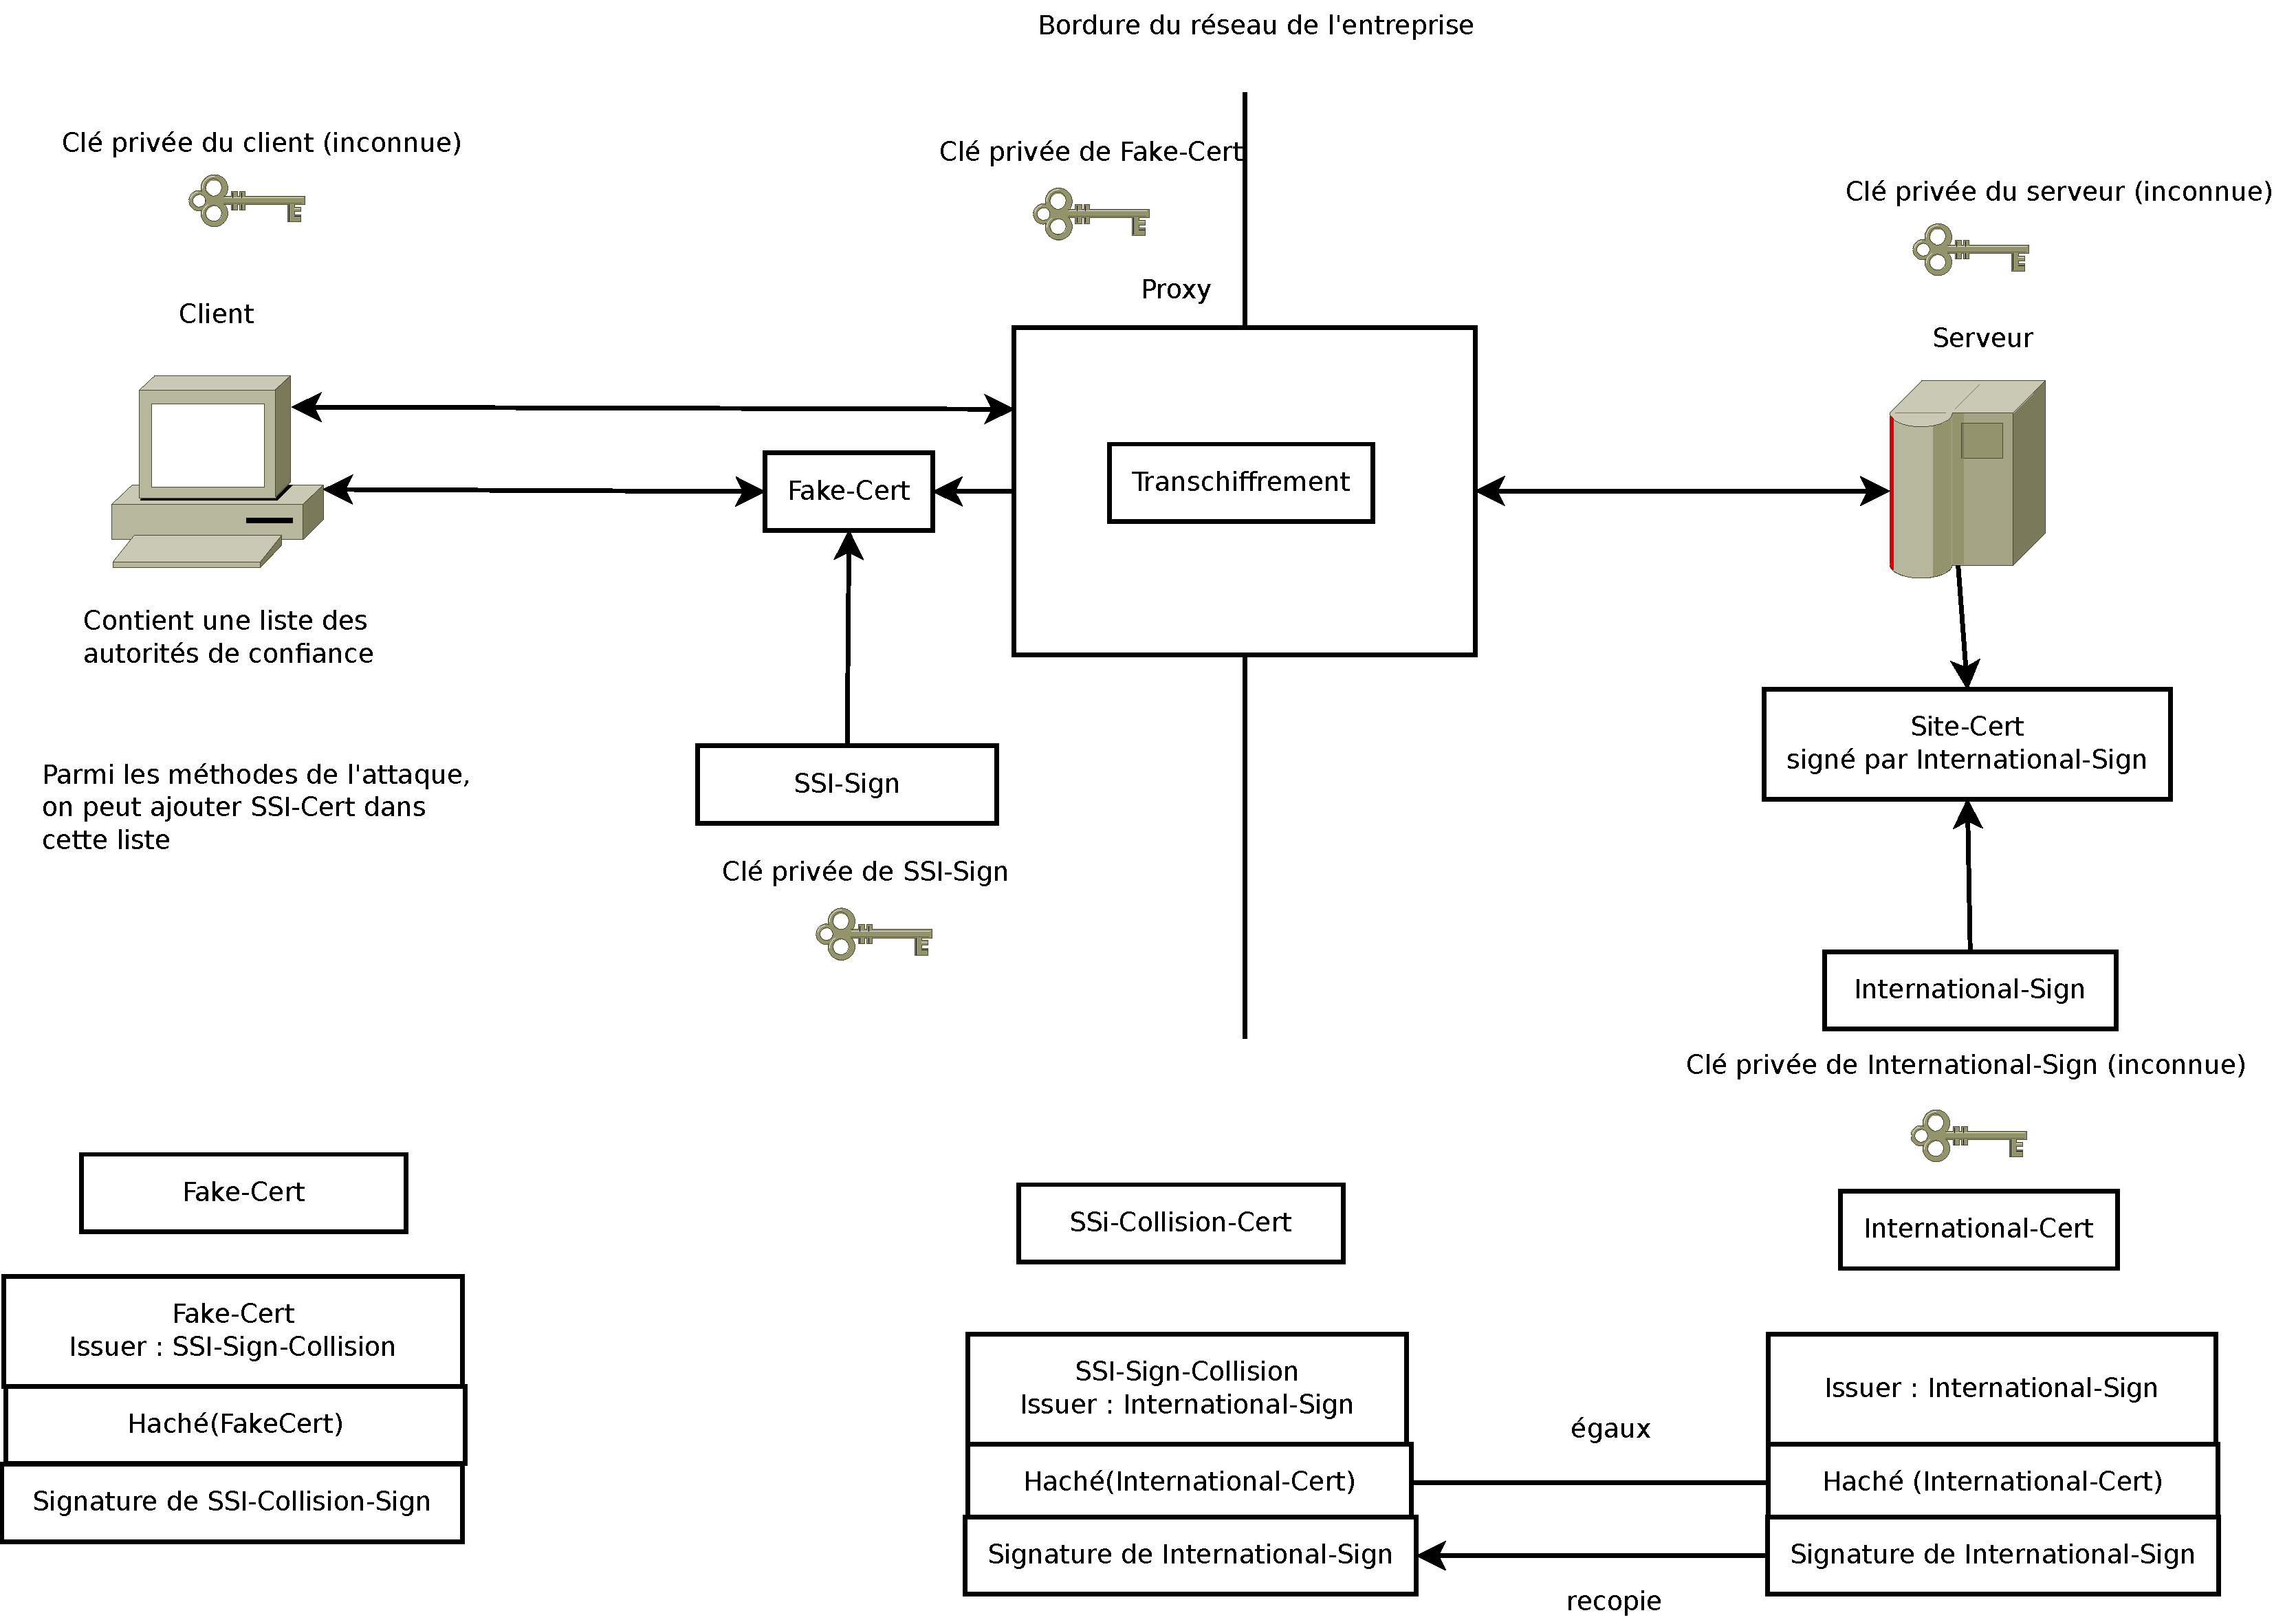
\includegraphics[width=\textwidth]{images/schema_autorites.pdf}

\end{document}